\documentclass[conference]{IEEEtran}
\usepackage{cite}
\usepackage[utf8]{inputenc}
\usepackage{amsmath,amssymb,amsfonts}
\usepackage{algorithm}
\usepackage{algorithmic}
\usepackage{listings}
\usepackage{graphicx}
\usepackage{forest}
\usepackage{textcomp}
\usepackage{ragged2e}
\usepackage{tikz}
\usepackage{hyperref}
\usepackage{appendix}
\usetikzlibrary{automata,positioning}
\def\BibTeX{{\rm B\kern-.05em{\sc i\kern-.025em b}\kern-.08em
    T\kern-.1667em\lower.7ex\hbox{E}\kern-.125emX}}

\title{Proyecto del curso Análisis y Diseño de Algoritmos}

\author{
	\IEEEauthorblockN{1\textsuperscript{st} Piero Morales Alcalde}
	\IEEEauthorblockA{
		\textit{Computer Science Student} \\
		\textit{Universidad de Ingeniería y Tecnología}\\
		Lima, Perú \\
		piero.morales@utec.edu.pe
	}
	\and
	\IEEEauthorblockN{2\textsuperscript{nd} André Segovia Melgarejo}
	\IEEEauthorblockA{
		\textit{Computer Science Student} \\
		\textit{Universidad de Ingeniería y Tecnología}\\
		Lima, Perú \\
		andre.segovia@utec.edu.pe
	}
	\and                                                                                                                                                              
	\IEEEauthorblockN{3\textsuperscript{rd} Osman Vilchez Aguirre}
	\IEEEauthorblockA{
		\textit{Computer Science Student} \\
		\textit{Universidad de Ingeniería y Tecnología}\\
		Lima, Perú \\
		osman.vilchez@utec.edu.pe
	}
}

\begin{document}

\maketitle

\section{Introduction}
En este proyecto se va resolver el problema de \textsc{Min-Matching} con el uso de algoritmos de tipo Greedy y con Programación dinámica.

\section{Problema de Min-Matching}

Dados dos vectores $A$ y $B$ de ceros y unos, se debe encontar un \textbf{matching de peso mínimo}. En cada uno de los vectores se pueden encontrar bloques. Un \textit{bloque} es un subarreglo de unos. Cada bloque puede ser denotado por un par ordenado $[i,j]$, donde $i$ es el índice inicial del bloque y $j$ es el índice final del bloque. Por ejemplo, si $A$ tiene $m$ bloques, entonces se pueden ordenar dichos bloques de forma creciente por índice inicial.\\\\
Ahora, se quiere asociar los segmentos de $A$ con los segmentos de $B$. Más formalmente, un \textit{matching} entre $A$ y $B$ es un conjunto $M$ de pares ordenados $(i,j)$ que comple las siguientes condiciones.\\
\begin{enumerate}
    \item Todo índice entre $1$ y $m$ aparece alguna vez en la primera coordenada de algún par ordenado en $M$. Todo índice entre $1$ y $n$ aparece alguna vez en la segunda coordenada de algún par ordenado en $M$.\\
    \item Si $(i_1,j_2) \in M$, $i_1<i_2$ y $j1<j2$, entonces $(i_2,j_1) \notin M$.\\
    \item Si $(i_1,j_1)$, $(i_2,j_2) \in M$ con $i_1<i_2$ y $j_1<j_2$, entonces $(i_1,j_2)$, $(i_2,j_1) \notin M$.\\
\end{enumerate}
Es decir, un \textit{matching} corresponde a una transformación entre bloques de $A$ hacia los bloques de $B$, tal que algunos bloques de $A$ son divididos y otros bloques son agrupados.\\\\
Formalmente, dado un \textit{matching} entre dos vectores, $A$ y un índice $i$, una i-división es un subconjunto $(i,j_1),(i,j_2),...,(i,j_k)$ del matching original. Note que, debido a la definición de matching, $j_1,j_2,...,j_k$ son índices consecutivos. Y dado un índice $j$, un j-agrupamiento es un subconjunto $(i_1,j),(i_2,j),...,(i_l,j)$ del matching original. Note que, debido a la definición de matching, $i_1,i_2,...,i_l$ son índices consecutivos.\\\\
Si $D=\{(i,j_1),(i,j_2),...,(i,j_k)\}$ es una división, entonces el peso asociado a dicha división es el siguiente.\\
\begin{center}
    $w\left(D\right)=\frac{\left|A_i\right|}{\left|B_{j_1}\right|+\left|B_{j_2}\right|+...+\left|B_{j_k}\right|}$
\end{center}
\verb| |\\
Si $D=\{(i_1,j),(i_2,j),...,(i_l,j)\}$ es una agrupación, entonces el peso asociado a dicha agrupación es la siguiente.\\
\begin{center}
    $w\left(D\right)=\frac{\left|A_{i_1}\right|+\left|A_{i_2}\right|+...+\left|A_{i_l}\right|}{\left|B_j\right|}$
\end{center}
\verb| |\\
El peso de un matching $M$, denotado por $w(M)$, es definido como la suma de los pesos de las agrupaciones y las divisiones en $M$, como se muestra a continuación.\\
\begin{center}
    $w\left(M\right)=\sum _{D:D\:es\:una\:division\:o\:agrupacion\:en\:M}\:w\left(D\right)$
\end{center}
\verb| |

\section{Pregunta 1: Algoritmo voráz}
Analise, diseñe e implemente un algoritmo voráz con complejidad
lineal para el problema \textsc{Min-Matching}. Su algoritmo no deberá encontrar necesariamente el matching de peso mínimo.\\\\
\textit{Entrada del algoritmo}: Dos arreglos $A$ y $B$ de ceros y unos de tamaño $p$, con $n$ bloques y $m$ bloques respectivamente (los valores de $n$ y $m$ no son recibidos como entrada).\\\\
\textit{Salida del algoritmo}: Un matching entre $A$ y $B$, no necesariamente óptimo, y su peso.\\\\
\textit{Tiempo de ejecución del algoritmo}: $O(max\{m,n\})$.\\\\
Como solución voráz al problema de \textsc{Min-Matching} primero se ha construido un algoritmo que convierte los dos vectores de unos y ceros iniciales en dos vectores de números enteros que se envían como argumentos al algoritmo principal.\\\\
El algoritmo para la conversión de vectores se muestra a continuación.

\newpage

\begin{algorithm}
\caption{\textsc{Convert-Vector}}
\begin{algorithmic}
\REQUIRE Un arreglo $A$ de unos y ceros.
\ENSURE Un arreglo $A'$ con la suma de unos para cada bloque.
\begin{flushleft}
\textsc{Convert-Vector}$(A)$
\end{flushleft}
    \STATE $count=0$
    \STATE $values=[\emptyset]$
    \FOR{$i$ in $A$}
        \IF{$i=1$}
            \STATE $count=count+1$
        \ELSE
            \IF{$count\neq0$}
                \STATE $values.add(count)$
                \STATE $count=0$
            \ENDIF
        \ENDIF
    \ENDFOR
    \IF{$count\neq0$}
        \STATE $values.add(count)$
    \ENDIF
    \RETURN $values$
\end{algorithmic}
\end{algorithm}

Luego de realizar la conversión de vectores de unos y ceros en vectores de número enteros, se puede pasar a realizar el matching entre los dos nuevos vectores. El algoritmo para este matching se detalla como \textsc{Min-Matching}.\\\\
Por ejemplo, supongamos que tenemos los siguientes vectores como entrada inicial.
\begin{center}
    $A=[0,1,1,1,0,0,1,0,1,1,0,1,1,0,1,1,1,0,1,0]$\\
    $B=[0,0,1,1,0,1,1,0,0,0,1,1,1,1,1,0,0,1,1,0]$
\end{center}
Cada uno de estos vectores se ejecutarían sobre el algoritmo \textsc{Convert-Vector}, el cual recibe como argumento un vector de unos y ceros. Luego de pasar ambos vectores sobre dicho algortimo, obtenemos como resultado los siguientes vectores de números enteros.
\begin{center}
    $A=[3,1,2,2,3,1]$\\
    $B=[2,2,5,2]$
\end{center}
Estos dos vectores, luego van a ser enviados como argumentos al algortimo principal \textsc{Min-Matching} que se va a encargar de hacer el matching entre estos dos vectores. Como el algortimo no necesariamente nos tiene que devolver el matching de peso mínimo, se puede hacer la siguiente elección voráz.\\\\
\textit{Elección voráz}: Realizar divisones y agrupamientos de forma intercalada desde el inicio hasta el final de los vectores, como se observa a continuación.\\
\begin{center}
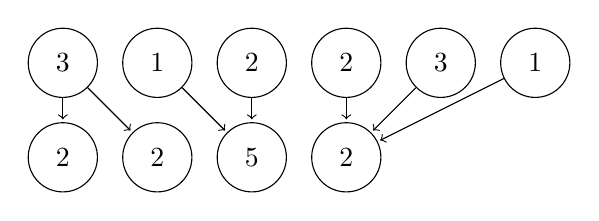
\begin{tikzpicture}[shorten >= 1pt, node distance = 1.2cm, on grid, auto] 
   \node[state] (q_0) {$3$};
   \node[state] (q_1) [right = of q_0] {$1$};
   \node[state] (q_2) [right = of q_1] {$2$};
   \node[state] (q_3) [right = of q_2] {$2$};
   \node[state] (q_4) [right = of q_3] {$3$};
   \node[state] (q_5) [right = of q_4] {$1$};
   \node[state] (q_6) [below = of q_0] {$2$};
   \node[state] (q_7) [right = of q_6] {$2$};
   \node[state] (q_8) [right = of q_7] {$5$};
   \node[state] (q_9) [right = of q_8] {$2$};
   \path[->]
    (q_0) edge node {} (q_6)
          edge node {} (q_7)
    (q_1) edge node {} (q_8)
    (q_2) edge node {} (q_8)
    (q_3) edge node {} (q_9)
    (q_4) edge node {} (q_9)
    (q_5) edge node {} (q_9);
\end{tikzpicture}
\end{center}

Para esta elección voraz se presentan las siguientes condiciones que hay que tener en cuenta.
\begin{itemize}
    \item Si los dos vectores de entrada ($A$ y $B$) son iguales,
        \begin{itemize}
            \item Si el tamaño de los vectores es multiplo de $3$.
            \item Si el tamaño de los vectores es multiplo de $3+1$.
            \item Si el tamaño de los vectores es multiplo de $3+2$.
        \end{itemize}
    \item Si las dos cadenas de entrada ($A$ y $B$) son diferentes.
\end{itemize}

Cuando se tiene dos vectores cuyo tamaño son múltiplos de 3, se puede hacer divisiones y agrupamientos de bloques de manera intercalada sin ningún problema. De esta manera, siempre se va a obtener \textit{i-divisiones} de la forma $(i,j_1),(i,j_2)$ y \textit{j-agrupamientos} de la forma $(i_1,j),(i_2,j)$, como se muestra a continuación.\\
\begin{center}
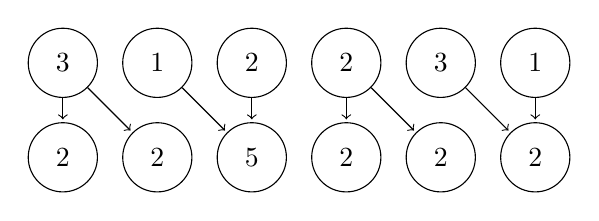
\begin{tikzpicture}[shorten >= 1pt, node distance = 1.2cm, on grid, auto] 
   \node[state] (q_0) {$3$};
   \node[state] (q_1) [right = of q_0] {$1$};
   \node[state] (q_2) [right = of q_1] {$2$};
   \node[state] (q_3) [right = of q_2] {$2$};
   \node[state] (q_4) [right = of q_3] {$3$};
   \node[state] (q_5) [right = of q_4] {$1$};
   \node[state] (q_6) [below = of q_0] {$2$};
   \node[state] (q_7) [right = of q_6] {$2$};
   \node[state] (q_8) [right = of q_7] {$5$};
   \node[state] (q_9) [right = of q_8] {$2$};
   \node[state] (q_10) [right = of q_9] {$2$};
   \node[state] (q_11) [right = of q_10] {$2$};
   \path[->]
    (q_0) edge node {} (q_6)
          edge node {} (q_7)
    (q_1) edge node {} (q_8)
    (q_2) edge node {} (q_8)
    (q_3) edge node {} (q_9)
          edge node {} (q_10)
    (q_4) edge node {} (q_11)
    (q_5) edge node {} (q_11);
\end{tikzpicture}
\end{center}
\verb| |\\
Para el caso cuando el tamaño de los vectores es un múltiplo de $3$ más $1$, al comienzo, se realizan las divisiones y agrupaciones de la misma manera, hasta que queden $4$ elementos por asignar. En este punto, se hace una división entre el primer elemento de $A$ que aún no ha sido asignado con todos los elementos sin asignar de $B$, menos el último. Luego, se hace una agrupación entre los elementos restantes de $A$ con el último elemento de $B$. Esta forma de match se muestra a continuación.\\
\begin{center}
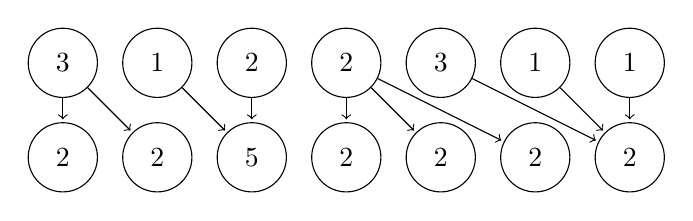
\begin{tikzpicture}[shorten >= 1pt, node distance = 1.2cm, on grid, auto] 
   \node[state] (q_0) {$3$};
   \node[state] (q_1) [right = of q_0] {$1$};
   \node[state] (q_2) [right = of q_1] {$2$};
   \node[state] (q_3) [right = of q_2] {$2$};
   \node[state] (q_4) [right = of q_3] {$3$};
   \node[state] (q_5) [right = of q_4] {$1$};
   \node[state] (q_6) [right = of q_5] {$1$};
   \node[state] (q_7) [below = of q_0] {$2$};
   \node[state] (q_8) [right = of q_7] {$2$};
   \node[state] (q_9) [right = of q_8] {$5$};
   \node[state] (q_10) [right = of q_9] {$2$};
   \node[state] (q_11) [right = of q_10] {$2$};
   \node[state] (q_12) [right = of q_11] {$2$};
   \node[state] (q_13) [right = of q_12] {$2$};
   \path[->]
    (q_0) edge node {} (q_7)
          edge node {} (q_8)
    (q_1) edge node {} (q_9)
    (q_2) edge node {} (q_9)
    (q_3) edge node {} (q_10)
          edge node {} (q_11)
          edge node {} (q_12)
    (q_4) edge node {} (q_13)
    (q_5) edge node {} (q_13)
    (q_6) edge node {} (q_13);
\end{tikzpicture}
\end{center}
\verb| |\\
Por último, para el caso cuando el tamaño de los vectores es un múltiplo de $3$ más $2$, al comienzo, se realizan las divisiones y agrupaciones de la misma manera que el caso 1, hasta que queden $5$ elementos por asignar. En este punto, se hace una división entre el primer elemento de $A$ que aún no ha sido asignado con todos los elementos sin asignar de $B$, menos el último. Luego, se hace una agrupación entre los elementos restantes de $A$ con el último elemento de $B$. Esta forma de match se muestra a continuación.\\
\begin{center}
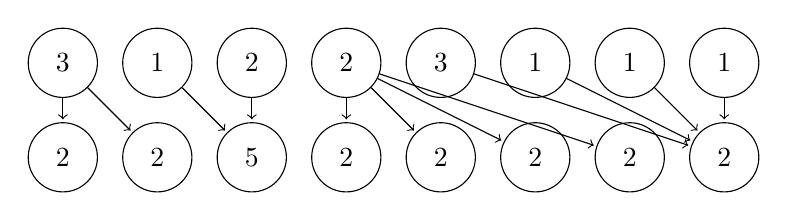
\begin{tikzpicture}[shorten >= 1pt, node distance = 1.2cm, on grid, auto] 
   \node[state] (q_0) {$3$};
   \node[state] (q_1) [right = of q_0] {$1$};
   \node[state] (q_2) [right = of q_1] {$2$};
   \node[state] (q_3) [right = of q_2] {$2$};
   \node[state] (q_4) [right = of q_3] {$3$};
   \node[state] (q_5) [right = of q_4] {$1$};
   \node[state] (q_6) [right = of q_5] {$1$};
   \node[state] (q_7) [right = of q_6] {$1$};
   \node[state] (q_8) [below = of q_0] {$2$};
   \node[state] (q_9) [right = of q_8] {$2$};
   \node[state] (q_10) [right = of q_9] {$5$};
   \node[state] (q_11) [right = of q_10] {$2$};
   \node[state] (q_12) [right = of q_11] {$2$};
   \node[state] (q_13) [right = of q_12] {$2$};
   \node[state] (q_14) [right = of q_13] {$2$};
   \node[state] (q_15) [right = of q_14] {$2$};
   \path[->]
    (q_0) edge node {} (q_8)
          edge node {} (q_9)
    (q_1) edge node {} (q_10)
    (q_2) edge node {} (q_10)
    (q_3) edge node {} (q_11)
          edge node {} (q_12)
          edge node {} (q_13)
          edge node {} (q_14)
    (q_4) edge node {} (q_15)
    (q_5) edge node {} (q_15)
    (q_6) edge node {} (q_15)
    (q_7) edge node {} (q_15);
\end{tikzpicture}
\end{center}

\newpage

Ahora, para los casos en los que los vectores tienen diferentes tamaños, se debe hacer una división de ambos vectores hasta que tengan el tamaño del vector menor menos $1$. Así, tendríamos dos vectores del mismo tamaño que se puede procesar con cualquiera de las maneras ya mencionadas. Y para los nodos restantes, quedarían hacer una divisón si es que el tamaño original del vector $A$ es menor que el tamaño original de $B$, y un agrupamiento en caso contrario, como se muestra a continuación.\\
\begin{center}
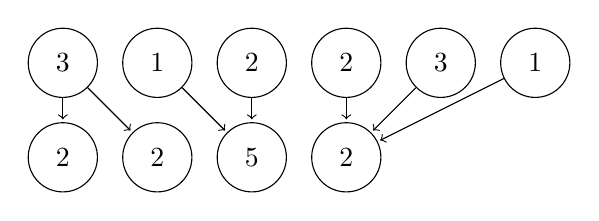
\begin{tikzpicture}[shorten >= 1pt, node distance = 1.2cm, on grid, auto] 
   \node[state] (q_0) {$3$};
   \node[state] (q_1) [right = of q_0] {$1$};
   \node[state] (q_2) [right = of q_1] {$2$};
   \node[state] (q_3) [right = of q_2] {$2$};
   \node[state] (q_4) [right = of q_3] {$3$};
   \node[state] (q_5) [right = of q_4] {$1$};
   \node[state] (q_6) [below = of q_0] {$2$};
   \node[state] (q_7) [right = of q_6] {$2$};
   \node[state] (q_8) [right = of q_7] {$5$};
   \node[state] (q_9) [right = of q_8] {$2$};
   \path[->]
    (q_0) edge node {} (q_6)
          edge node {} (q_7)
    (q_1) edge node {} (q_8)
    (q_2) edge node {} (q_8)
    (q_3) edge node {} (q_9)
    (q_4) edge node {} (q_9)
    (q_5) edge node {} (q_9);
\end{tikzpicture}
\end{center}

El pseudocódigo de este algoritmo voraz para el problema se muestra en el algoritmo 2 \textsc{Min-Matching-Voraz}.

\begin{algorithm}
\caption{\textsc{Min-Matching-Voraz}}
\begin{algorithmic}
\REQUIRE Dos arreglos $A$ y $B$ con la suma de unos por bloque.
\ENSURE Un matching entre $A$ y $B$, y su peso.
\begin{flushleft}
\textsc{Min-Matching-Voraz}$(A,B)$
\end{flushleft}
    \STATE $result=\emptyset$
    \IF{$A.length=B.length$}
        \IF{$A.length$ $mod$ $3=0$}
            \STATE $result=$ \textsc{Match-Mult-3}$(A,B)$
        \ELSIF{$A.length$ $mod$ $3=1$}
            \STATE $result=$ \textsc{Match-Mult-3-1}$(A,B)$
        \ELSE
            \STATE $result=$ \textsc{Match-Mult-3-2}$(A,B)$
        \ENDIF
    \ELSE
        \IF{$A.length>B.length$}
            \STATE $A'=A[1:B.length-1]$
            \STATE $B'=B[1:B.length-1]$
            \IF{$A'.length$ $mod$ $3=0$}
                \STATE $result=$ \textsc{Match-Mult-3}$(A',B')$
            \ELSIF{$A'.length$ $mod$ $3=1$}
                \STATE $result=$ \textsc{Match-Mult-3-1}$(A',B')$
            \ELSE
                \STATE $result=$ \textsc{Match-Mult-3-2}$(A',B')$
            \ENDIF
            \STATE $t=A[B.length:A.length]$
            \STATE $result.add(t,B[B.length])$
        \ELSE
            \STATE $A'=A[1:A.length-1]$
            \STATE $B'=B[1:A.length-1]$
            \IF{$A'.length$ $mod$ $3=0$}
                \STATE $result=$ \textsc{Match-Mult-3}$(A',B')$
            \ELSIF{$A'.length$ $mod$ $3=1$}
                \STATE $result=$ \textsc{Match-Mult-3-1}$(A',B')$
            \ELSE
                \STATE $result=$ \textsc{Match-Mult-3-2}$(A',B')$
            \ENDIF
            \STATE $t=A[A.length:B.length]$
            \STATE $result.add(A[A.length],t)$
        \ENDIF
    \ENDIF
\end{algorithmic}
\end{algorithm}

\section{Pregunta 2: Recurrencia}
Tenemos la siguiente recurrencia para el problema de \textsc{Min-Matching}.\\
\begin{center}
$OPT(i,j)$
\begin{math}
  \resizebox{.8\hsize}{!}{
  \left\{
    \begin{array}{l}
      \frac{A_i}{\sum _{k=1}^iB_k} \text{ for all } i=1\\\\
      \frac{\sum _{k=1}^iA_k}{B_j} \text{ for all } j=1\\\\
      min(min_{l=1}^{j-1}\{OPT(i-1,j-l)+\frac{A_i}{\sum _{k=j-l+1}^jB_k}\};\\
      min_{l=1}^{i-1}\{OPT(i-l,j-1)+\frac{\sum _{k=i-l+1}^iA_k}{B_j}\}) \text{ otherwise}
    \end{array}
  \right.}
\end{math}
\end{center}
\section{Pregunta 3: Recursivo}
\subsection{Recurrencia de complejidad}
Tenemos la siguiente recurrencia de complejidad para el problema de \textsc{Min-Matching-Recursivo}.\\
\begin{center}
$C(m,n)$
\begin{math}
  \resizebox{.8\hsize}{!}{
  \left\{
    \begin{array}{l}
      $2*c_1$ \text{ for all } i=2 j=2\\\\
      C\left(m;n\right)=\sum _{n=1}^{n-1}C\left(m-1;n-h\right)+\\\\
        \sum _{n=1}^{m-1}C\left(m-h;n-1\right)+\Omega \left(1\right) \text{ otherwise}
    \end{array}
  \right.}
\end{math}
\end{center}

\subsection{Demostración de complejidad}
Tenemos lo siguiente:\\\\
$C\left(m;n\right)=\sum _{n=1}^{n-1}C\left(m-1;n-h\right)+$\\\\
$\sum _{n=1}^{m-1}C\left(m-h;n-1\right)+\Omega \left(1\right)\ge C\left(m-1;n-1\right)+$\\\\
$C\left(m-1;n-1\right)$\\

$\therefore C\left(m;n\right)\ge C\left(m-1;n-1\right)+C\left(m-1;n-1\right)$

\[
 \boxed{C\left(m;n\right)\ge 2C\left(m-1;n-1\right)}
 \]

\textit{Hipótesis}: $C\left(m;n\right)=\Omega \left(2^r\right)$, $r$ es máximo\\
$\Rightarrow \:C\left(m;n\right)\ge \:C\cdot \:2^r\:\leftrightarrow \:m\:\wedge \:n\:\ne \:1$\\\\

\textit{Adicional}:
$C\left(2;2\right)=2\cdot K\ge 2^2\cdot C$\\
$k=2\:\wedge \:C=1$\\

\begin{align*}
   C\left(2;2\right)&=\Omega \left(2^2\right) \\
   &\vdots\\
   C\left(m-1;n-1\right)&=\Omega \left(2^{r-1}\right)\\
   C\left(m;n\right)&=\Omega \left(2^r\right)
\end{align*}

\newpage

Por hipótesis inductiva, tenemos:\\\\
$C\left(m;n\right)\ge 2\cdot C\left(m-1;n-1\right)$\\\\
$2^r\cdot K\ge 2\cdot 2^{r-1}\cdot K_1$\\\\
$K\cdot \:2\:\wedge \:K_1=1$ \textbf{Se verifica}\\\\
$C\left(m;n\right)=\Omega \:\left(2^{max\left\{m,n\right\}}\right);\:m\:\wedge \:n \neq 1$

\subsection{Algoritmo recursivo}
Para resolver el problema de \textsc{Min-Matching} se ha planteado el siguiente pseudocódigo.
\begin{algorithm}
\caption{\textsc{Min-Matching-Recursivo}}
\begin{algorithmic}
\REQUIRE Dos arreglos $A$ y $B$ con la suma de unos por bloque.
\ENSURE Un matching entre $A$ y $B$, y su peso.
\begin{flushleft}
\textsc{Min-Matching-Recursivo}$(A,B)$
\end{flushleft}
    \STATE $i=A.length$
    \STATE $j=B.length$
    \IF{$i=1$ \AND $j=1$}
        \RETURN $\{(A[i],B[j])\}$
    \ELSIF{$i=1$ \OR $j=1$}
        \IF{$i=1$}
            \STATE $match=(A[i],\emptyset)$
            \FOR{$a=1$ to $j+1$}
                \STATE $match[2].add(B[a])$
            \ENDFOR
            \RETURN $\{match\}$
        \ELSE
            \STATE $match=(\emptyset,B[j])$
            \FOR{$a=1$ to $i+1$}
                \STATE $match[1].add(A[a])$
            \ENDFOR
            \RETURN $\{match\}$
        \ENDIF
    \ELSE
        \STATE $pesos=\emptyset$
        \STATE $match=$ \textsc{Min-Matching-Recursivo}$(A[1:i],B[1:j])$
        \STATE $match.add(A[i],B[j])$
        \STATE $pesos.add(match)$
        \FOR{$a=1$ to $i$}
            \STATE $matches=$ \textsc{Min-Matching-Recursivo}$(A[1:a],B[1:j])$
            \STATE $match=(\emptyset,B[j])$
            \FOR{$b=a$ to $i+1$}
                \STATE $match[1].add(A[b])$
            \ENDFOR
            \STATE $matches.add(match)$
            \STATE $pesos.add(matches)$
        \ENDFOR
        \FOR{$a=2$ to $j$}
            \STATE $matches=$ \textsc{Min-Matching-Recursivo}$(A[1:i],B[1:a])$
            \STATE $match=(A[i],\emptyset)$
            \FOR{$b=a$ to $j+1$}
                \STATE $match[2].add(B[b])$
            \ENDFOR
            \STATE $matches.add(match)$
            \STATE $pesos.add(matches)$
        \ENDFOR
    \RETURN $min(pesos)$
    \ENDIF
\end{algorithmic}
\end{algorithm}
\verb| |\\
\section{Pregunta 4: Memorizado}

\subsection{Arbol de análisis de costo}

\begin{center}
    \begin{forest}
for tree={l sep-=.7em,l=0},
[\scalebox{0.7}{
$\begin{array}{c}
M(m,n)
\end{array}$}
 [\scalebox{0.7}{
$\begin{array}{c}
min(m-1,n'-1)
\end{array}$}
  [\scalebox{0.7}{
$\begin{array}{c}
M(m-1,1) \text{...}
\end{array}$}
  ]
  [\scalebox{0.7}{
$\begin{array}{c}
\text{...} M(m-1,n-1)
\end{array}$}
  ]
 ]
 [\scalebox{0.7}{
$\begin{array}{c}
min(m'-1,n-1)
\end{array}$}
  [\scalebox{0.7}{
$\begin{array}{c}
M(1,n-1) \text{...}
\end{array}$}
  ]
  [\scalebox{0.7}{
$\begin{array}{c}
\text{...} M(m-1,n-1)
\end{array}$}
  ]
 ]
]
\end{forest}
\end{center}
\begin{align*}
   &\vdots
\end{align*}
\begin{FlushRight}
    \begin{forest}
for tree={l sep-=.7em,l=0},
[\scalebox{0.7}{
$\begin{array}{c}
M(m-(n-1),1)
\end{array}$}
 [\scalebox{0.7}{
$\begin{array}{c}
M(1,1) \text{...}
\end{array}$}
 ]
 [\scalebox{0.7}{
$\begin{array}{c}
\text{...} M(m-n+1,1)
\end{array}$}
 ]
]
\end{forest}
\end{FlushRight}

\subsection{Recurrencia de complejidad}
Tenemos la siguiente recurrencia para el problema de \textsc{Min-Matching-Memorizado}.\\
\begin{center}
$C(m,n)$
\begin{math}
  \resizebox{.8\hsize}{!}{
  \left\{
    \begin{array}{l}
      c_1*n \text{ for all } i=1\\\\
      c_1*m \text{ for all } j=1\\\\
      C(m-1,n-1) + k(n-2)+d \text{  otherwise} 
    \end{array}
  \right.}
\end{math}
\end{center}

\subsection{Demostración de complejidad}
\text{Suponiendo que} $m>n$ :\\ \\
\begin{math}
    C(m,n) = C(m-1,n-1) + k(m-2)+ d\\
    =C(m-2,n-2)+k(m-2)+k(m-3)+2d\\
    =C(m-2,n-2)+2km-k(2+3)+2d\\
    =C(m-3,n-3)+3km-k(2+3+4)+3d\\
    \vdots\\
    =C(m-(n-1),n-(n-1))+ (n-1)km-\\ k(2+3+4...+n)+(n-1)d\\
    =C(m-(n-1),1)+(n-1)km-k(\frac{n*(n+1)}{2}-1)+(n-1)d\\
    =O(m)+(n-1)km+O(n^2)+O(n) 
\end{math}\\ \\
\text{Se verifica que }$O(m)$, $O(n)$ y $O(n^2)$ son $O(m*n)$\\
\text{Entonces: }\\
Faltaría demostrar que $(n-1)km = O(m*n)$\\ 
\begin{math}
    k*nm-k*m \leq c*mn\\
    k-\frac{k}{n} \leq c \\
    \text{Con c = 1 }n_0\text{=1; } n \geq n_0 >0\\
    0 \leq c \\
    \Rightarrow (n-1)km = O(n*m) \\ \\
    \textbf{Conluimos: } 
    C(m,n) = O(n*m)
\end{math}

\begin{algorithm}
\caption{\textsc{Min-Matching-Memoizado}}
\begin{algorithmic}
\REQUIRE Dos arreglos $A$ y $B$ con la suma de unos por bloque.
\ENSURE Un matching entre $A$ y $B$, y su peso.
\begin{flushleft}
\textsc{Min-Matching-Memoizado}$(A,B)$
\end{flushleft}
    \STATE $i=A.length$
    \STATE $j=B.length$
    \IF{$i=1$ \AND $j=1$}
        \RETURN $\{(A[i],B[j])\}$
    \ELSIF{$i=1$ \OR $j=1$}
        \IF{$i=1$}
            \STATE $match=(A[i],\emptyset)$
            \FOR{$a=1$ to $j+1$}
                \STATE $match[2].add(B[a])$
            \ENDFOR
            \RETURN $\{match\}$
        \ELSE
            \STATE $match=(\emptyset,B[j])$
            \FOR{$a=1$ to $i+1$}
                \STATE $match[1].add(A[a])$
            \ENDFOR
            \RETURN $\{match\}$
        \ENDIF
    \ELSE
        \IF{$memoria.get(i)$}
            \IF{$memoria[i].get(j)$}
                return $memoria[i][j]$
            \ENDIF
        \ENDIF
        \STATE $pesos=\emptyset$
        \STATE $match=$ \textsc{Min-Matching-Memorizado}$(A[1:i],B[1:j])$
        \STATE $match.add(A[i],B[j])$
        \STATE $pesos.add(match)$
        \FOR{$a=2$ to $i$}
            \STATE $matches=$ \textsc{Min-Matching-Memorizado}$(A[1:a],B[1:j])$
            \STATE $match=(\emptyset,B[j])$
            \FOR{$b=a$ to $i+1$}
                \STATE $match[1].add(A[b])$
            \ENDFOR
            \STATE $matches.add(match)$
            \STATE $pesos.add(matches)$
        \ENDFOR
        \FOR{$a=2$ to $j$}
            \STATE $matches=$ \textsc{Min-Matching-Memorizado}$(A[1:i],B[1:a])$
            \STATE $match=(A[i],\emptyset)$
            \FOR{$b=a$ to $j+1$}
                \STATE $match[2].add(B[b])$
            \ENDFOR
            \STATE $matches.add(match)$
            \STATE $pesos.add(matches)$
        \ENDFOR
        \STATE $minp = min(pesos)$
        \IF{$memoria.get(i)$}
            \STATE $memoria[i][j] = minp$
        \ELSE
            \STATE $memoria[i] = dic()$
            \STATE $memoria[i][j] = minp$
        \ENDIF
        \RETURN $memoria[i][j]$
    \ENDIF
\end{algorithmic}
\end{algorithm}

\renewcommand{\appendixname}{Anexos}
\renewcommand{\appendixtocname}{Anexos}
\renewcommand{\appendixpagename}{Anexos}

\appendix
Link repositorio GitHub: \href{https://github.com/Piero16301/Proyecto_ADA.git}{\underline{Proyecto ADA}}

\end{document}